\documentclass[12pt]{article}
\usepackage{letltxmacro}
\usepackage{makeidx}
\usepackage{multirow}
\usepackage{multicol}
\usepackage[dvipsnames,svgnames,table]{xcolor}
\usepackage{graphicx}
\usepackage{epstopdf}
\usepackage{ulem}
\usepackage{hyperref}
\usepackage{amsmath}
\usepackage{amssymb}
\usepackage{lipsum}
\usepackage{setspace}

\title{}
\usepackage[paperwidth=595pt,paperheight=841pt,top=72pt,right=72pt,bottom=72pt,left=72pt]{geometry}

\makeatletter
	\newenvironment{indentation}[3]%
	{\par\setlength{\parindent}{#3}
	\setlength{\leftmargin}{#1}       \setlength{\rightmargin}{#1}%
	\advance\linewidth -\leftmargin       \advance\linewidth -\rightmargin%
	\advance\@totalleftmargin\leftmargin  \@setpar{{\@@par}}%
	\parshape 1\@totalleftmargin \linewidth\ignorespaces}{\par}%
	
\makeatother 

% new LaTeX commands

\renewcommand{\baselinestretch}{1.5} 
\renewcommand*{\familydefault}{\rmdefault}
\begin{document}

\pagenumbering{gobble}
\vspace{4cm}
\begin{center}
\begin{indentation}{0pt}{0pt}{0pt}
\textbf{{\Large EFFICIENT BANDWIDTH UTILISATION IN WIRELESS MESH NETWORKS}}
\end{indentation}
\end{center}

\vspace{0.5cm}

\begin{center}
\begin{indentation}{0pt}{0pt}{0pt}
{\normalsize{\textbf {\textit {Submitted by}}}}
\end{indentation}
\end{center}
\vspace{0.5cm}

\begin{center}
\begin{indentation}{0pt}{0pt}{0pt}
{\normalsize \bf ASHISH GUPTA}
\end{indentation}
\end{center}

\begin{center}
\begin{indentation}{0pt}{0pt}{0pt}
{\normalsize \bf CHANDRIKA PARIMOO}
\end{indentation}
\end{center}

\begin{center}
\begin{indentation}{0pt}{0pt}{0pt}
{\normalsize \bf RUTUJA SHAH}
\end{indentation}
\end{center}

\begin{center}
\begin{indentation}{0pt}{0pt}{0pt}
{\normalsize \bf SUDIPTO CHATTERJEE}
\end{indentation}
\end{center}
\vspace{1cm}

\begin{center}
\begin{indentation}{0pt}{0pt}{0pt}
{\normalsize \bf Pune Institute of Computer Technology}
\end{indentation}
\end{center}

\begin{center}
\begin{indentation}{0pt}{0pt}{0pt}
{\normalsize \bf Team ID: BQOS179}
\end{indentation}
\end{center}

\pagebreak


\begin{indentation}{0pt}{0pt}{0pt}
\textbf{{{\Large Introduction}}}
\end{indentation}
\vspace{0.5cm}
\begin{indentation}{0pt}{0pt}{0pt}
{\normalsize \hspace{1cm} Wireless Mesh Networks(WMN) have been emerging in the last couple of years as a cost effective alternative to traditional wired access networks. A typical WMN combines a fixed network (backbone) and a mobile network (backhaul). The nodes in a WMN often act as relays, forwarding traffic to or from other mesh nodes, or providing localized connectivity to mobile or pervasive wireless devices, such as laptops, desktops and other mobile clients. Some of these nodes, called mesh gates, act as gateways that are directly connected to the Internet. Among the various variants of mesh networks, IEEE 802.11s is the IEEE standard for Wireless Mesh Networks and is also present in the Linux kernel. This project uses o11s (open80211s), which is the implementation of IEEE 802.11s in the Linux kernel, as the underlying mesh network.}
\end{indentation}

\begin{indentation}{0pt}{0pt}{0pt}
{\normalsize \hspace{1cm}Currently, in o11s, every mesh node is associated with a maximum of one mesh gate. This type of single association involves the entire traffic being directed towards the mesh gate. The gate's available bandwidth is shared by all its clients, and consequently, the throughput per client is reduced with an increase in the number of clients. Additionally, constraints such as the mesh gate being common to many outbound paths reduce the effective link capacity due to the multipoint-to-point nature of the traffic.}
\end{indentation}
\begin{indentation}{0pt}{0pt}{0pt}
{\normalsize \hspace{1cm}This project aims to improve the utilization of total available bandwidth by using multiple Internet access gateways inside a Wireless Mesh Network instead of the usual association with a single Internet gateway. This is achieved transparently without any changes to applications using the mesh. Traffic sensitive load sharing is also incorporated for the selection of gateways.}
\end{indentation}

\begin{indentation}{0pt}{0pt}{0pt}
{\normalsize \hspace{1cm}The benefits include increased network throughput as well as reduced network setup costs as the need for additional network hardware is eliminated.}
\end{indentation}

\begin{indentation}{0pt}{0pt}{0pt}
\vspace{1cm}
\textbf{{{\Large Problem Statement}}}
\end{indentation}
\vspace{0.5cm}

\begin{indentation}{0pt}{0pt}{0pt}
{\normalsize \hspace{1cm} Enhance bandwidth utilization in Wireless Mesh Networks using a decentralized approach to improve throughput.}
\end{indentation}

\begin{indentation}{0pt}{0pt}{0pt}
\vspace{1cm}
\pagebreak
\textbf{{{\Large Solution}}}
\end{indentation}
\vspace{0.5cm}
\begin{indentation}{0pt}{0pt}{0pt}
{\normalsize \hspace{1cm} The devised solution makes use of all gateways present in the Wireless Mesh Network. The packets are categorized on a per flow basis and not on a per packet basis as it helps us not worry about deep packet inspection in order to determine the correct path. Since a single flow of packets is categorized by open ports in the sender as well as the receiver, we use the source port on the sender as a unique key for relating to a specific flow. This helps preserve the sanity of applications as well as meet their expectations of seeing all packets of the same flow on the same port.}
\end{indentation}


\begin{indentation}{0pt}{0pt}{0pt}
{\normalsize \hspace{1cm} A gate is a machine which is connected to the mesh network using a wireless interface and has an internet connection available on another interface. Both these interfaces are bridged in order to make use of both the mesh capabilities as well as the Internet capabilities simultaneously. The gate broadcasts it's ability to perform as a gate by periodically sending out L2 packets containing it's IP address among other metrics. Traffic originating within the mesh network which is destined for an external network is routed using one of the available gates. The gateway is selected based on metrics such as the hop count and available link capacity. Traffic destined for the local network is not routed through the gate, and never leaves the local network.} 
\end{indentation}

\begin{indentation}{0pt}{0pt}{0pt}
{\normalsize \hspace{1cm}While the total and available bandwidth help in deciding the load on the mesh gate, the latency which also takes into account the hop count while routing to the gateway is a critical factor in routing http and VoIP traffic. Network capacity can increase linearly with the number of gateways only with proper load balancing and resource provisioning. This kind of proper association, which prevents the formation of bottlenecks and distributes the network load evenly realizes the linear capacity increase.}
\end{indentation}


\begin{indentation}{0pt}{0pt}{0pt}
{\normalsize \hspace{1cm} Through experimental setups using Click modular router it is demonstrable that unless the underlying hardware link capacity becomes the bottleneck, linear gain in the network takes place.}
\end{indentation}

\pagebreak
\begin{indentation}{0pt}{0pt}{0pt}
\vspace{1cm}
\textbf{{{\Large Presentation}}}
\end{indentation}
\vspace{0.5cm}
\begin{indentation}{0pt}{0pt}{0pt}
{\normalsize \hspace{1cm} In order to verify the working of this scheme, we will present it using four machines. The Client, C, has access to two other machines (the gates, G1 and G2) which in turn can access the fourth machine, the server S. This scenario effectively replicates the setup on an Internet enabled network where a client has access to two internet connections, both of which lead to a specific server somewhere on the Internet. The client does not have direct access to the server's resources as it is enforced using scripts on the client.}
\end{indentation}

\begin{indentation}{0pt}{0pt}{0pt}
{\normalsize \hspace{1cm} A fixed set of unchanging files will be downloaded from the server to the client using three path combinations. The first being only via G1, C - G1 - S. The second path used was only via G2, C - G2 - S. The third path used both the paths, C - G1, G2 - S,  through the gates to fetch those files. Comparing the time required to download the files via the above three paths will prove the aim of our project.}
\end{indentation}

\begin{indentation}{0pt}{0pt}{0pt}
{\normalsize \hspace{1cm} Another demonstration includes using two connections at the same time, a bittorrent client will be able to achieve higher download speeds compared to when using a single connection. This proves that this solution is applicable to real networks and will help the users exploit all available bandwidth on the network which would otherwise be left unused.}
\end{indentation}

\vspace{1cm}

\begin{figure}[h]
  \centering
    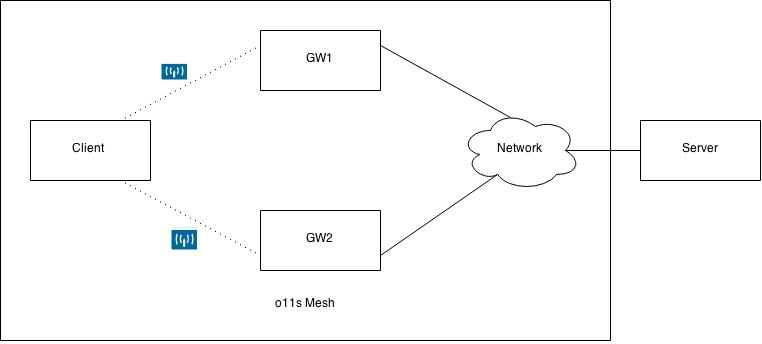
\includegraphics[scale=0.50]{ExperimentLayout}
    \caption{Presentation to show linear gain in the network.}
    \label{Diagram: Presentation layout}
\end{figure}

\pagebreak

\begin{indentation}{0pt}{0pt}{0pt}
\textbf{{{\Large References}}}
\end{indentation}

\vspace{1.5cm}

\begin{indentation}{0pt}{0pt}{0pt}
[1] I. F. Akyildiz, X. Wang, and W. Wang, “Wireless mesh networks: a survey,” Computer Network. ISDN Syst., vol. 47, pp.
\end{indentation}

\vspace{1cm}

\begin{indentation}{0pt}{0pt}{0pt}
[2] Mihail L. Sichitiu Dept. of  Electrical and Computer Engineering, North Carolina State 
University, “Wireless Mesh Networks : Opportunities and Challenges”.
\end{indentation}

\vspace{1cm} 

\begin{indentation}{0pt}{0pt}{0pt}
[3] Vishal Sevani, Bhaskaran Raman, CS Dept, IIT Bombay, “Understanding HTTP traffic performance in TDMA mesh networks”.
\end{indentation}

\vspace{1cm}

\begin{indentation}{0pt}{0pt}{0pt}
[4] Franesco Paolo Déila, Giovanni Di Stasi, Stefao Stallone, Roberto Canonico , niversito di Napoli Federico, Napoli, “Bittorrent traffic optimization in Wireless Mesh Networks”.
\end{indentation}

\vspace{1cm}

\begin{indentation}{0pt}{0pt}{0pt}
[5] Hiertz, G.R.Denteneer, D.Max, S.Taori, R.Cardona, J.Berlemann, L.Walke, "IEEE 802.11s: The WLAN Mesh Standard", Wireless Communications, IEEE  (Volume:17 ,  Issue: 1 ),February 2010
\end{indentation}

\vspace{1cm}

\begin{indentation}{0pt}{0pt}{0pt}
[6] Madhusudan Singh, Song-Gon Lee2, HoonJae Lee "Non-root-based Hybrid Wireless Mesh Protocol for Wireless Mesh Networks", International Journal of Smart Home Vol. 7, No. 2, March, 2013
\end{indentation}

\vspace{1cm}

\begin{indentation}{0pt}{0pt}{0pt}
[7] Mohammed I. Gumel, Nasir Faruk and A.A. Ayeni, "ROUTING WITH LOAD BALANCING IN WIRELESS MESH NETWORKS", International Journal of Current Research Vol. 3, Issue, 7, pp.087-092, July, 2011
\end{indentation}

\vspace{1cm}

\begin{indentation}{0pt}{0pt}{0pt}
[8] open80211s [Online] Available: www.github.com/open80211s.
\end{indentation}
\end{document}



